\documentclass[12pt]{article}
\usepackage{amsmath,amssymb,amsthm}
\usepackage{graphicx}
\usepackage[margin=1in]{geometry}
\usepackage{fancyhdr}
\usepackage{tikz}

\usepackage{tikz}
\usetikzlibrary{shapes, positioning}


\begin{figure}
\centering
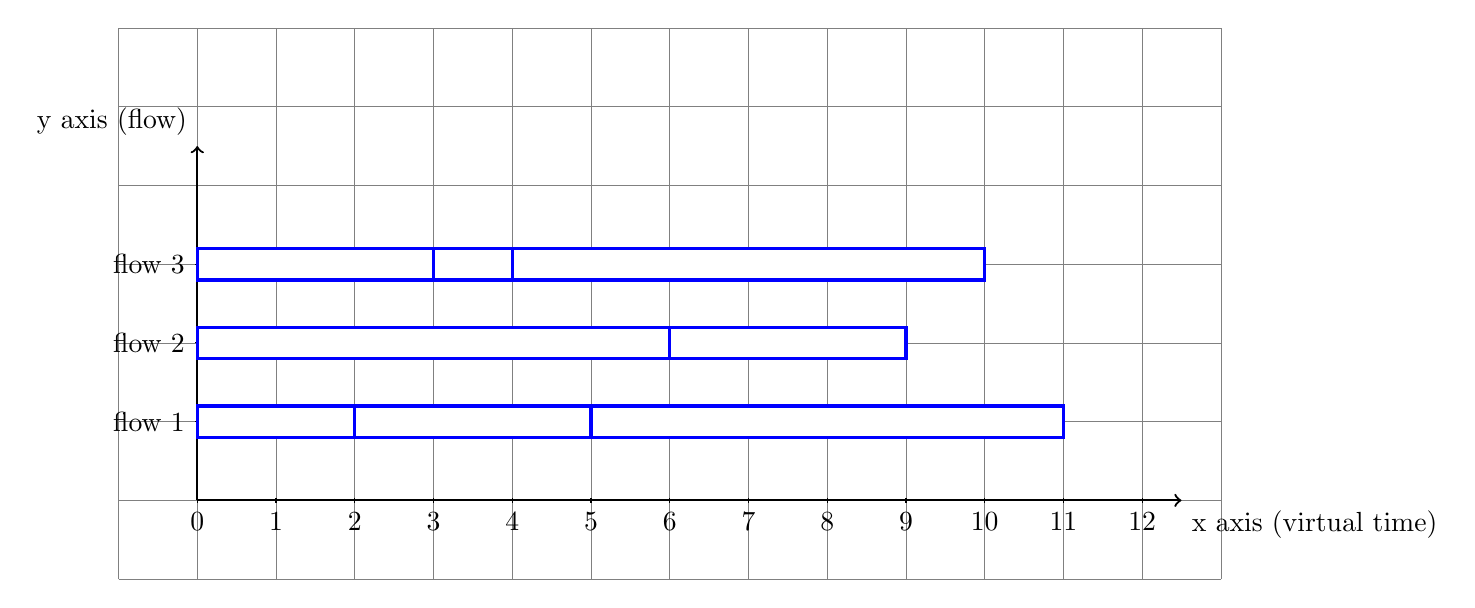
\begin{tikzpicture}

% draw the cordinator

%% draw grid
\draw[step=1cm,gray,very thin] (-1,-1) grid (13,6);

%% draw x axis and y axis
\draw[thick,->] (0,0) -- (12.5,0) node[anchor=north west] {x axis (virtual time)};
\draw[thick,->] (0,0) -- (0,4.5) node[anchor=south east] {y axis (flow)};

%% label x & y axis 
\foreach \x in {0,...,12}
    \draw (\x cm,1pt) -- (\x cm,-1pt) node[anchor=north] {$\x$};
\foreach \y in {1,2,3}
    \draw (1pt,\y cm) -- (-1pt,\y cm) node[anchor=east] {flow $\y$};


% flow 1
\filldraw[fill=white, draw=blue,very thick] (0,0.8) rectangle (2,1.2);
\filldraw[fill=white, draw=blue,very thick] (2,0.8) rectangle (5,1.2);
\filldraw[fill=white, draw=blue,very thick] (5,0.8) rectangle (11,1.2);

% flow 2
\filldraw[fill=white, draw=blue,very thick] (0,1.8) rectangle (6,2.2);
\filldraw[fill=white, draw=blue,very thick] (6,1.8) rectangle (9,2.2);

% flow 3
\filldraw[fill=white, draw=blue,very thick] (0,2.8) rectangle (3,3.2);
\filldraw[fill=white, draw=blue,very thick] (3,2.8) rectangle (4,3.2);
\filldraw[fill=white, draw=blue,very thick] (4,2.8) rectangle (10,3.2);

\end{tikzpicture}
\end{figure}

\end{document}